\section{Bestehende Lösungen}
Es gibt einige bestehende Ansätze, die die verschiedenen Aspekte des direktionalen Hörens auf technische Apparaturen übertragen. Diesen begegnen wir in unserem alltäglichen Leben relativ häufig. Die einfachste Form eines solchen Verfahrens ist das Richtmikrofon. Dieses führt allerdings keine aktive Ortung durch, sondern kann Schall lediglich aus einer bestimmten Richtung besonders gut den aufnehmen. Um diese Fähigkeit für eine Richtungsbestimmung zu nutzen, müsste man also das Richtmikrofon drehen, oder es auf eine andere Weise aktiv nach der Schallquelle ausrichten. Ein weiterer Ansatz, dem wir in unserem alltäglichen Leben noch sehr viel häufiger begegnen, steckt in fast allen Mobiltelefonen. Diese filtern beim Telefonieren verschiedene Umgebungsgeräusche aus dem Mikrofonsignal, um die Sprachqualität zu verbessern. Die hierzu verwendeten Verfahren sind allerdings meist eher einfach gehalten und erlauben keine Bestimmung der Herkunftsrichtung eines Geräusches. Das Resultat dieses Verfahrens ähnelt sehr dem eines Richtmikrofons. Bei dieser Technik erfolgt ein Teil der Geräuschunterdrückung bei der Signalverarbeitung, also nach der eigentlichen Schallwandlung durch das Mikrofon. Hierdurch unterscheidet sich dieser Ansatz deutlich von dem des Richtmikrofones. Allerdings können auch mithilfe dieser Störgeräuschunterdrückung noch keine Positionen ermittelt werden. Auch moderne Hörgeräte verwenden ein ähnliches Verfahren, welches auch bei einer größeren Distanz zwischen Mikrofon und Schallquelle funktioniert und der gesuchten Lösung somit näher kommt. Sowohl die Geräuschunterdrückung in Handys als auch die Filtertechniken in Hörgeräten verwenden oft zwei oder drei Mikrofone.\\
\begin{wrapfigure}{r}{0.5\textwidth}
    \centering
    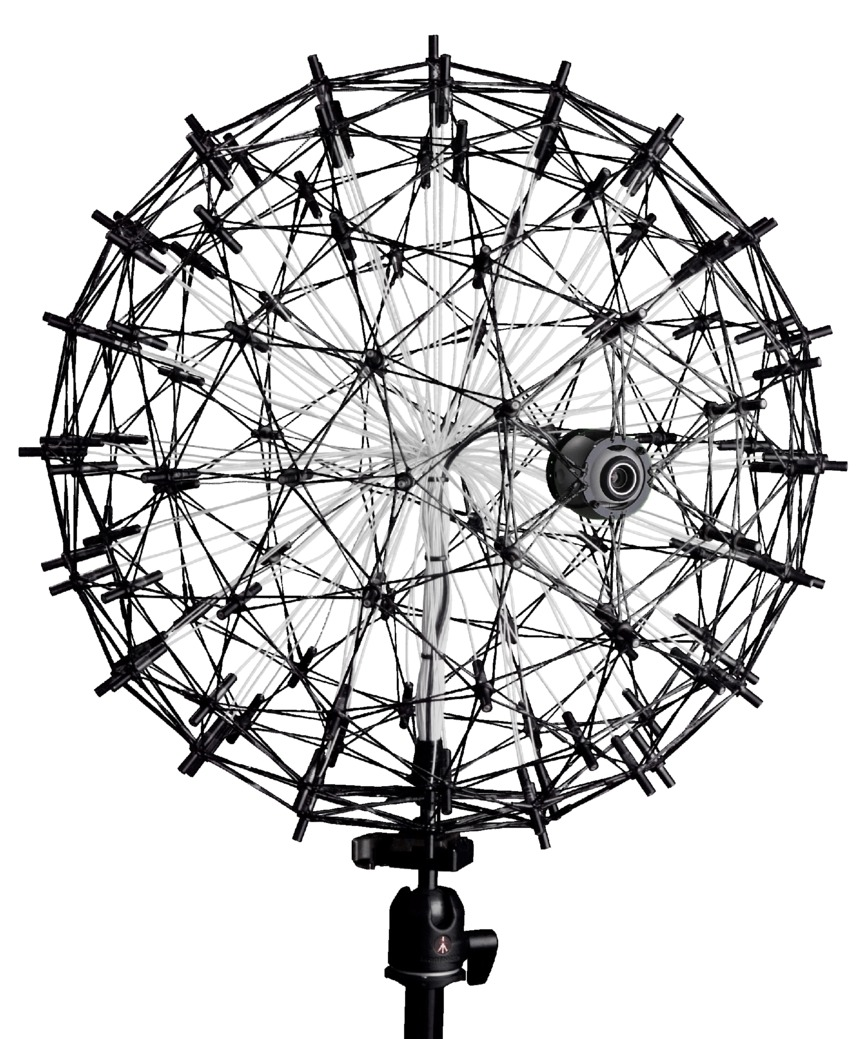
\includegraphics[width=0.5\linewidth]{img/akusticCamera}
    \caption{Beispiel für eine akustische Kamera~\cite{camera}\label{fig:camera}}
\end{wrapfigure}
Eine andere existierende Lösung ist die akustische Kamera (siehe Abb.~\ref{fig:camera}). Sie wird dazu verwendet, lärmemittierende Positionen an Produkten zu finden, um diese optimieren zu können~\cite{camera}. Die akustische Kamera verwendet allerdings bedeutend mehr Mikrofone als die anderen Verfahren. Einige Modelle arbeiten mit mehr als \num{350} Mikrofone~\cite{nmics}. Außerdem können bestehende akustische Kameras nicht in andere technische Kontexte eingebettet werden und sind so nicht universell einsetzbar, da sie an die Auswertungssoftware des Kameraherstellers gebunden sind und stark auf ihren jeweiligen Anwedungszweck optimiert sind.\\
Da uns alle vorhandenen Lösungen nicht zufrieden gestellt haben, wollten wir ein eigenes Verfahren für die akustische Richtungsbestimmung entwickeln, das schon mit einer geringen Anzahl von Mikrofonen eine vollständige Richtungsbestimmung ermöglicht und leicht erweiterbar auf zusätzliche Auswertungsschritte ist.
